\documentclass{article}

\usepackage{siunitx}
\usepackage{graphicx}
\usepackage{tikz}
\usepackage{pgfplots}

\usepgfplotslibrary{dateplot}
\usepgfplotslibrary{units}

\begin{document}
\begin{tikzpicture}

\node (ssn) at (0,0) {
	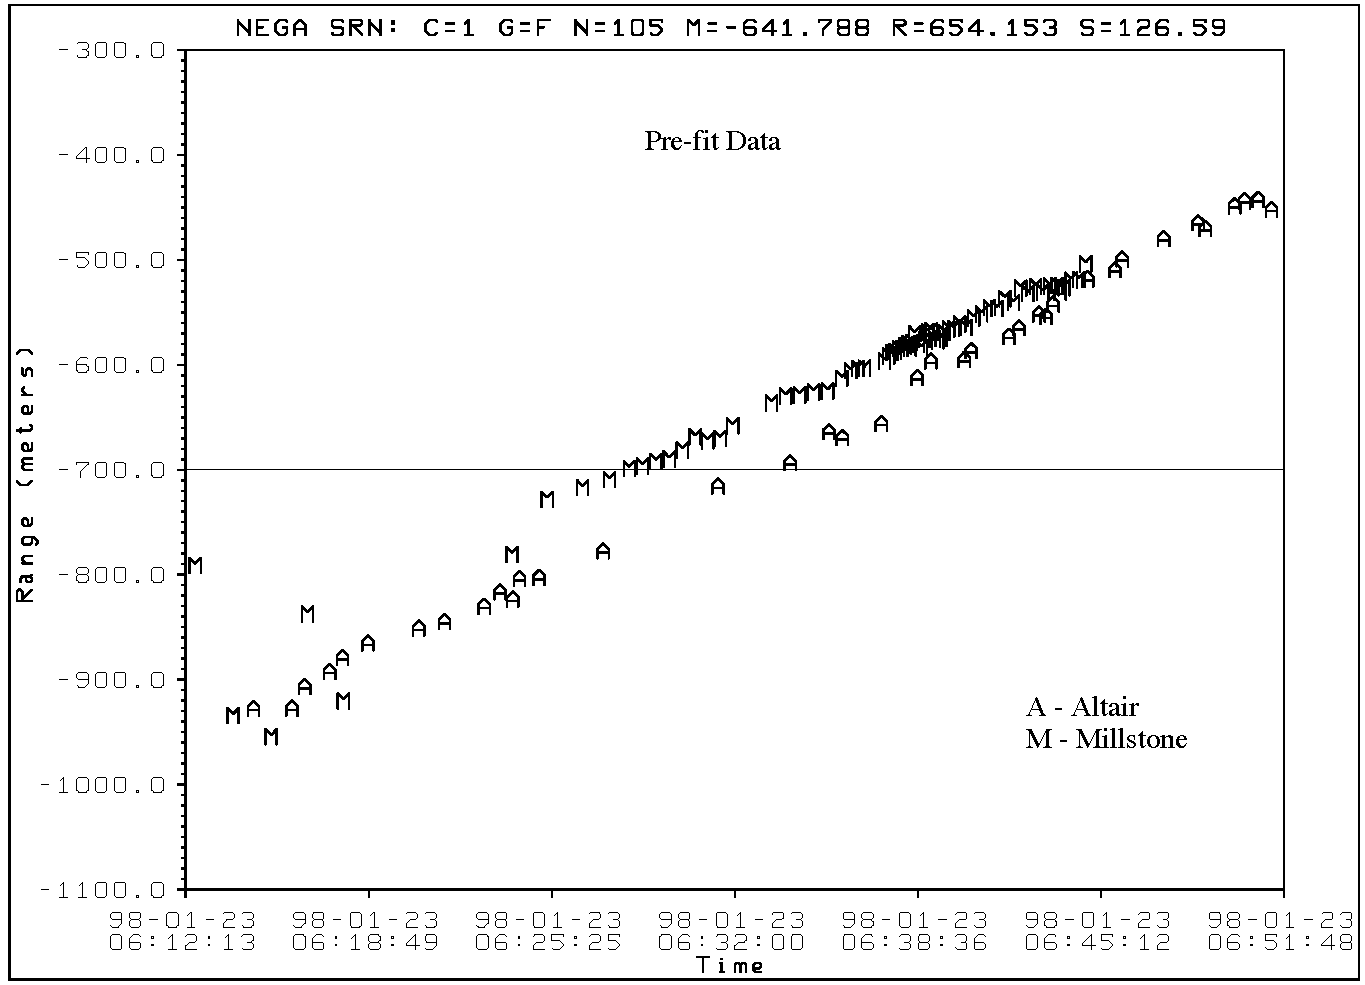
\includegraphics[width=.9\textwidth] {Antreasian/fig10_near_SSNrange.pdf}
	};

\node (jplh) at (-0.37,-0.25) {
	\begin{tikzpicture}
		[ xscale = 1.2825, yscale = 1.18 ]
	\footnotesize
	\begin{axis} [
		date coordinates in = x,
		date ZERO=1998-01-23,
		xmin={1998-01-23 06:12:00},
		xmax={1998-01-23 06:52:00},
		scaled ticks = false,
		tick align = inside,
		xtick pos = left,
		xticklabel = {\tiny \hour:\minute},
		xticklabel style = {anchor = south, color = blue},
		%
		ymax = -300,
		ymin = -1100,
		ytick pos = left,
		minor y tick num = 0,
		yticklabel = {\tiny ~\pgfmathprintnumber{\tick} \si{\metre}},
		yticklabel style = {anchor = west, color = blue},
		ylabel = {},
		%
		grid = none,
		legend style={
			at = {(0.50,0.30)},
			anchor = north,
			draw = none,
			font = \tiny,
			fill = none
			}
		]

		\addplot [mark = none, blue,
			y filter/.code={\pgfmathparse{\pgfmathresult-25}}
			]
			table [x index=0, y index=7, col sep=tab, skip first n=1]
			{../near/near_altair.t};

		\addlegendentry[blue] {$\Delta r$-25 for ALTAIR (\si{\metre})};

		\addplot [mark = none, red]
			table [x index=0, y index=7, col sep=tab, skip first n=1,
				restrict y to domain=-1100:-500
			]
			{../near/near_millstone.t};

		\addlegendentry[red] {$\Delta r$ for Millstone (\si{\metre})};

		\addplot [mark = none, blue, dotted,
			y filter/.code={\pgfmathparse{\pgfmathresult-50}}
			]
			table [x index=0, y index=7, col sep=tab, skip first n=1]
			{../near/near_altair.t};

		\addplot [mark = none, blue, dotted]
			table [x index=0, y index=7, col sep=tab, skip first n=1]
			{../near/near_altair.t};

		\addlegendentry[blue] {\SI{\pm 25}{\metre} bounds for ALTAIR};

		\addplot [mark = none, red, dotted,
			y filter/.code={\pgfmathparse{\pgfmathresult-5}}
			]
			table [x index=0, y index=7, col sep=tab, skip first n=1,
				restrict y to domain=-1100:-500
			]
			{../near/near_millstone.t};

		\addplot [mark = none, red, dotted,
			y filter/.code={\pgfmathparse{\pgfmathresult+5}},
			]
			table [x index=0, y index=7, col sep=tab, skip first n=1,
				restrict y to domain=-1100:-500
			]
			{../near/near_millstone.t};

		\addlegendentry[red] {\SI{\pm 5}{\metre} bounds for Millstone};

	\end{axis}
	\begin{axis} [
		date coordinates in = x,
		date ZERO=1998-01-23,
		xmin={1998-01-23 06:12:00},
		xmax={1998-01-23 06:52:00},
		scaled ticks = false,
		tick align = inside,
		xtick pos = left,
		xticklabel = {\tiny \hour:\minute},
		xticklabel style = {anchor = south, color = blue},
		%
		minor y tick num = 0,
		ylabel = {},
		yticklabel = {\tiny ~\pgfmathprintnumber{\tick} \si{\kilo\metre}},
		yticklabel shift = -0.1cm,
		yticklabel style = {anchor = east, color = red},
		y filter/.code = {\pgfmathparse{1e-3*\pgfmathresult}},
		axis y line* = right,
		%
		grid = none,
		legend style={
			at = {(0.50,0.85)},
			anchor = north,
			draw = none,
			font = \tiny,
			fill = none
			}
		]

		\addplot [mark = none, dashed, blue]
			table [x index=0, y index=4, col sep=tab, skip first n=1]
			{../near/near_altair.t};

		\addlegendentry[blue] {$r$ for ALTAIR (\si{\kilo\metre})};

		\addplot [mark = none, dashed, red]
			table [x index=0, y index=4, col sep=tab, skip first n=1]
			{../near/near_millstone.t};

		\addlegendentry[red] {$r$ for Millstone (\si{\kilo\metre})};
	\end{axis}
	\end{tikzpicture}
	};
\end{tikzpicture}
\end{document}
